\documentclass[11pt, a4paper]{article}

% Set the title of the current document to be produced.
\newcommand{\doctitle}{Neural Networks}
% Command for the due date of the homework.
\newcommand{\duedate}{\color{rltred}{\faCalendarCheckO { }Due date: May 1st, before midnight \faCalendarCheckO	}}

%------------------------------------------------------------
% Import commands for both teacher and course information.  | 
% NOTE: Change your teacher and course info in these files. |
%------>------>------>------>------>------>------>------>-->|
\newcommand{\instructor}{Lin Nan} 
\newcommand{\college}{Shanghai Jiao Tong University}
\newcommand{\semester}{Summer 2022}
\newcommand{\coursetitle}{Neural Networks} 
\newcommand{\coursenumber}{PRP}                              %|   
%
%------------------------------------------------------------
%-- Import packages and custom command definitons.          |
%------>------>------>------>------>------>------>------>-->|
%----------------------------------------------------
% The following is a list of LaTeX packages imports |
%------->------>------>------>------>------>---->---|
%

% The margins at the bottom of the page has been reduced.
% this allows for a slim footer.
\usepackage[left=1in,right=1in,top=1in,bottom=0.7in]{geometry}
% Original size:
%\usepackage[inner=1.5cm,outer=1.5cm,top=1.5cm,bottom=.5cm,margin=1in]{geometry}
\usepackage[
    colorlinks,
    pagebackref,
    pdfusetitle,
    urlcolor=blue,
    citecolor=blue,
    linkcolor=blue,    
    plainpages=false]
{hyperref}            
% ftp://ftp.dante.de/tex-archive/fonts/bbding/bbding.pdf
%https://ctan.math.illinois.edu/fonts/bbding/bbding.pdf
\usepackage{fancyhdr, lastpage, bbding, pmboxdraw}
\usepackage{fancyvrb}
\PassOptionsToPackage{usenames,dvipsnames}{xcolor}
\usepackage{acronym}
\usepackage{amsthm}
\usepackage{caption}
\usepackage{xcolor}
\usepackage{enumitem}
\usepackage{tabularx}
\usepackage{sectsty}
% pifont package doc at: https://ctan.math.ca/tex-archive/macros/latex/required/psnfss/psnfss2e.pdf
% pifont is used to define custom list and style list items using the \ding command. 
\usepackage{pifont} 
% bclogo used for making a colored box for notes. 
% @see: https://ctan.org/pkg/bclogo?lang=en
\usepackage[tikz]{bclogo} 
\usepackage{titlesec}  
\usepackage[open,openlevel=1]{bookmark}
\usepackage[UTF8]{ctex}
%-- @see http://ctan.sharelatex.com/tex-archive/fonts/fontawesome/doc/fontawesome.pdf
% Font Awesome  http://ctan.math.washington.edu/tex-archive/fonts/fontawesome5/doc/fontawesome5.pdf
% https://muug.ca/mirror/ctan/fonts/fontawesome5/doc/fontawesome5.pdf
\usepackage{fontawesome5}
%---------------------------------
% ==== Font setup.
% Load any of the following fonts.
%---------------------------------
%\usepackage{lmodern}
%\usepackage{mathptmx}
\usepackage{times}
%\usepackage[sc]{mathpazo} % Palatino font.
%\linespread{1.05} % Palatino needs more leading (space between lines)
\usepackage{tgbonum} % For Bonum/Bookman font.
\usepackage[utf8]{inputenc}
\usepackage[T1]{fontenc}
%---------------------------------
\usepackage{booktabs} 

\pagestyle{empty}
\usepackage{graphicx}
\usepackage{multicol}
\usepackage{blindtext}  
\usepackage{vhistory} % for making a table for the revision history.

\usepackage{float}

\usepackage{tcolorbox}
                                  %|  
%--------------------------------------------------------
%--> \customhrule: makes a customized rule whose width  | 
%                  should be passed as parameter.       |
%--------------------------------------------------------
\newcommand{\customhrule}[1]{
	\rule[1.4pt]{\linewidth}{#1}
}
%------------------------------------------------------
%--> \doublerule: makes a double rule.                |
%------------------------------------------------------ 
\newcommand{\doublerule}[1][.4pt]{
	\noindent
	\makebox[0pt][l]{\rule[.7ex]{\linewidth}{#1}}%
	\rule[1pt]{\linewidth}{#1}\par} 
%===== Custom Ruler commands  ==================
\renewcommand{\headrulewidth}{1pt}
\renewcommand{\footrulewidth}{0.4pt}

% Disable spaces between list items in a labeled list.
\setlist{noitemsep}
 
%-------------------------------------------------------------
%= The followig are declaraions of custom Lists              =
%-------------------------------------------------------------
%
%======= Green rectangles list =======================
% \Rectangle from bbind
\newlist{greenrectangles}{itemize}{4}
%\setlist[greenrectangles]{topsep=4pt,partopsep=0pt,itemsep=3pt,parsep=0pt,labelindent=0.5cm,leftmargin=*}
\setlist[greenrectangles]{itemsep=5pt,parsep=0pt,topsep=4pt,partopsep=3pt}
\setlist[greenrectangles,1]{font=\color{darkred},label={\color{darkgreen}{\Rectangle}}}

%======= Alphabetical  list =======================
\newlist{alphalist}{enumerate}{9}
\setlist[alphalist]{topsep=4pt,partopsep=0pt,itemsep=3pt,parsep=0pt,labelindent=0.5cm,leftmargin=*}
\setlist[alphalist,1]{label=\textbf{\alph*)}}
%======= Non-numbered list =======================
\newlist{itemizedlist}{itemize}{9}
\setlist[itemizedlist]{topsep=4pt,partopsep=0pt,itemsep=3pt,parsep=0pt,labelindent=0.5cm,leftmargin=*}
%\setlist[itemizedlist,1 ]{label=\textbf{\alph*)}}

%======= Arrowed list =======================
\newlist{arrows}{itemize}{4}
\setlist[arrows]{topsep=4pt,partopsep=0pt,itemsep=3pt,parsep=0pt,labelindent=0.5cm,leftmargin=*}
\setlist[arrows,1]{font=\color{darkred},label={\HandRight}}

%======= Bordered square list =======================
% Colorize the selected symbol? 
% ❏
\newlist{borderedsquare}{itemize}{4}
\setlist[borderedsquare]{topsep=4pt,partopsep=0pt,itemsep=3pt,parsep=0pt,labelindent=0.5cm,leftmargin=*}
\setlist[borderedsquare,1]{label=\ding{111}}

%======= Filled, curved arrow list =======================
\newlist{curveddarrow}{itemize}{4}
\setlist[curveddarrow]{topsep=4pt,partopsep=0pt,itemsep=3pt,parsep=0pt,labelindent=0.5cm,leftmargin=*}
\setlist[curveddarrow,1]{label=\small\faMarker}

%======= Colored pen list ======================= 
\newlist{coloredPen}{itemize}{4}
\setlist[coloredPen]{topsep=4pt,partopsep=0pt,itemsep=3pt,parsep=0pt,labelindent=0.5cm,leftmargin=*}
\setlist[coloredPen,1]{font=\color{darkred},label=\small\faMarker}

%======= Objectives list ======================= 
% ➠
\newlist{objectives}{itemize}{4}
\setlist[objectives]{topsep=4pt,partopsep=0pt,itemsep=3pt,parsep=0pt,labelindent=0.5cm,leftmargin=*}
\setlist[objectives,1]{label=\small\ding{224}}

%======= Dark starred list ======================= 
% ✸
\newlist{filledstarlist}{itemize}{4}
\setlist[filledstarlist]{topsep=4pt,partopsep=0pt,itemsep=3pt,parsep=0pt,labelindent=0.5cm,leftmargin=*}
\setlist[filledstarlist,1]{label=\small\ding{88}}

%======= Dark-bordered empty circle list ======================= 
% ❍
\newlist{emptyCircleList}{itemize}{4}
\setlist[emptyCircleList]{topsep=4pt,partopsep=0pt,itemsep=3pt,parsep=0pt,labelindent=0.5cm,leftmargin=*}
\setlist[emptyCircleList,1]{label=\small\ding{109}}

%======= Filled right arrow list ======================= 
% ➤
\newlist{filledRightArrowList}{itemize}{4}
\setlist[filledRightArrowList]{topsep=4pt,partopsep=0pt,itemsep=3pt,parsep=0pt,labelindent=0.5cm,leftmargin=*}
\setlist[filledRightArrowList,1]{label=\small\ding{228}}

%======= Numbered list: non-filled circle list ======================= 
% ➀
\newlist{numberedEmptyList}{itemize}{9}
\setlist[numberedEmptyList]{topsep=4pt,partopsep=0pt,itemsep=3pt,parsep=0pt,labelindent=0.5cm,leftmargin=*}
\setlist[numberedEmptyList,9]{label=\ding{182}}

%======= Right hand pointing list =======================
\newlist{rightHandPointingList}{itemize}{4}
\setlist[rightHandPointingList]{topsep=4pt,partopsep=0pt,itemsep=3pt,parsep=0pt,labelindent=0.5cm,leftmargin=*}
\setlist[rightHandPointingList,1]{font=\color{darkred},label={\HandRight}}

%----------------------------------------------------------------------
%=   The followig are custom colors declaraions                       |
%--  more colors codes can be found at: http://latexcolor.com/        | 
%-- usage: {\color{declared-color} some text}.                        |    
%  e.g.,: {\color{darkblue}{ This text will appear darkblue-colored}} |
%----------------------------------------------------------------------
\definecolor{darkblue}{rgb}{0,0,.6}
\definecolor{darkred}{rgb}{.7,0,0}
\definecolor{darkgreen}{rgb}{0,.6,0}
\definecolor{darkestred}{rgb}{.8,.1,0}
\definecolor{red}{rgb}{.98,0,0}
\definecolor{OliveGreen}{cmyk}{0.64,0,0.95,0.40}
\definecolor{CadetBlue}{cmyk}{0.62,0.57,0.23,0}
\definecolor{lightlightgray}{gray}{0.93}
\definecolor{vanierred}{RGB}{210,0,2}
\definecolor{darkestblue}{rgb}{0.0, 0.0, 0.55}
\definecolor{darkblue}{rgb}{0,0,.6}
\definecolor{darkred}{rgb}{.7,0,0}
\definecolor{darkgreen}{rgb}{0,.6,0}
\definecolor{darkestred}{rgb}{.8,.1,0}
\definecolor{red}{rgb}{.98,0,0}
\definecolor{OliveGreen}{cmyk}{0.64,0,0.95,0.40}
\definecolor{CadetBlue}{cmyk}{0.62,0.57,0.23,0}
\definecolor{lightlightgray}{gray}{0.93}
\definecolor{darkorange}{rgb}{255,140,0}
\definecolor{fluorescentyellow}{rgb}{0.8, 1.0, 0.0}
\definecolor{darkyellow}{rgb}{1,1,0.34}
\definecolor{lightyellow}{rgb}{1,1,0.6}
\definecolor{coolblack}{rgb}{0.0, 0.18, 0.39}
\definecolor{lightgray}{rgb}{.9,.9,.9}
\definecolor{darkgray}{rgb}{.4,.4,.4}
\definecolor{purple}{rgb}{0.65, 0.12, 0.82}
\definecolor{gray}{rgb}{0.4,0.4,0.4}
\definecolor{cyan}{rgb}{0.0,0.6,0.6}
\definecolor{dkgreen}{rgb}{0,0.6,0}
\definecolor{gray}{rgb}{0.5,0.5,0.5}
\definecolor{mauve}{rgb}{0.58,0,0.82}
\definecolor{lightblue}{rgb}{0.0,0.0,0.9}
\colorlet{punct}{red!60!black}
\definecolor{background}{HTML}{EEEEEE}
\definecolor{delim}{RGB}{20,105,176}
\colorlet{numb}{magenta!60!black}
\definecolor{coolblack}{rgb}{0.0, 0.18, 0.39}
\definecolor{forestgreen}{rgb}{0.0, 0.27, 0.13}
\definecolor{firebrick}{rgb}{0.7, 0.13, 0.13}
\definecolor{rltred}{rgb}{0.75,0,0}
\definecolor{rltgreen}{rgb}{0,0.5,0}
\definecolor{rltblue}{rgb}{0,0,0.75}
\definecolor{indigo}{rgb}{0.0, 0.25, 0.42}
\definecolor{jazzberryjam}{rgb}{0.65, 0.04, 0.37}
\definecolor{lava}{rgb}{0.81, 0.06, 0.13}
\definecolor{royalblue}{rgb}{0.0, 0.14, 0.4}
\definecolor{prussianblue}{rgb}{0.0, 0.19, 0.33}
\definecolor{prune}{rgb}{0.44, 0.11, 0.11}
\definecolor{cerisepink}{rgb}{0.93, 0.23, 0.51}
\definecolor{oxfordblue}{rgb}{0.0, 0.13, 0.28}
\definecolor{crimsonglory}{rgb}{0.75, 0.0, 0.2}
\definecolor{fireenginered}{rgb}{0.81, 0.09, 0.13}

%============================
% Commands for inserting colored text.
\newcommand{\bluetext}[1]{\textcolor{darkblue}{#1}}
\newcommand{\redtext}[1]{\textcolor{jazzberryjam}{#1}}

%=================================================================================================
% Command for styling tabled row header (left, center or right)
% Usage example: \thead{<Header text 1>} & \thead{<Header 2>} & \thead{<Header 3>} & \thead{<Header 4>} 
\newcommand*{\thead}[1]{\multicolumn{1}{l}{\bfseries #1}}	

%--------------------------------------------------
% ==== Doc header and footer setup.               |
%-------------------------------------------------- 
\renewcommand{\thefootnote}{\fnsymbol{footnote}}
\pagestyle{fancyplain}
\fancyhf{}
%- Disable the horizontal ruler in the header section.
\renewcommand{\headrulewidth}{0pt}
\rfoot{\fancyplain{}{page \thepage\ of \pageref{LastPage}}}
\cfoot{{\tiny{\college { } - { } \semester} }}
\lfoot{{\tiny{ \coursenumber -\coursetitle} }}
%- TODO: move the header content here.
\fancyfoot[RO, LE] {{\tiny{page \thepage\ of \pageref{LastPage} }}}
\thispagestyle{plain}
%------------------------------------------------------------

\newcolumntype{L}[1]{>{\raggedright\arraybackslash}p{#1}}
\newcolumntype{C}[1]{>{\centering\arraybackslash}p{#1}}
\newcolumntype{R}[1]{>{\raggedleft\arraybackslash}p{#1}}

%-- Spacing commands ------ 
\newcommand{\vspbpara}{\vspace*{.09in}}    
\newcommand{\customvspace}{\vspace{.5cm}}    
\titlespacing{\section}{0pt}{12pt}{9pt}
%-----
\newcommand{\vtitlespacing}{\vskip 0.3cm}
\newcommand{\paragraphentry}[1]{\noindent \textbf{\Large \underline{#1}} }
   
%
%---> Genereate & inject metadata describing                |
%     the produced document                                 |
%--------------------------------------------------------------
%-- Set up the hyperref package.                              |
%-- Generate and inject metadate in the produced PDF document |
%------>------>------>------>------>------>------>------>-->---
 \hypersetup{pdfauthor={\instructor},%
    pdftitle={\coursetitle},%
    pdfsubject={\doctitle},%
    pdfkeywords={\college},%
    pdfproducer={LaTeX},%
    pdfcreator={pdfLaTeX},
    bookmarks,
    bookmarksnumbered = true,
    bookmarksopen     = true,
    pdfpagelabels     = true,
    pdfstartview={XYZ null null 1.2}
}                                  %|
%------------------------------------------------------------

\topmargin      -60pt

\begin{document} 
    
%-------------------------------------------------------------
%-- Make the header of the document                          |
%------>------>------>------>------>------>------>------>--> |
%--------------------------------------------------------------------------
%- The following produces the document header including the title.        |
%- The document header includes: the college/university name, faculty,    |
%  department, course number and title as well as the assignment/homework | 
%  title and due date.                                                    | 
%-------------------------------------------------------------------------|
%
\noindent % <-- need to have this first.
%
\begin{minipage}{.40\textwidth}
    {\color{darkred} \faSchool} { \textsc{\college}}{ } {\color{darkred} \faSchool}\\ 
    \small\textsc{ \semester}
\end{minipage}%
\hfill	
\begin{minipage}{0.60\textwidth}%
    \raggedleft%
    {\Large \textsc{\coursetitle}\par}
    \doublerule % insert a double rule.
    \textsc{Author}: \instructor\\
\end{minipage}%
\vspace{2.8cm}
{
    %--> Insert homework title and due date.
    \hrule\vspace{.2cm}
    \centering
    {\scshape 
        \Large \color{darkestblue}{\doctitle}\par}
    \vspace{.3cm}    
}

\vspace{1.2cm}


\vskip .3in
%
\tableofcontents

\clearpage

%-------------------------------------------------------------
%-- Begin here!                          |
%------>------>------>------>------>------>------>------>--> |

\section{Bases}
\subsection{Architectures}
\begin{figure}[H] %h:当前位置, t:顶部, b:底部, p:浮动页
    \centering
    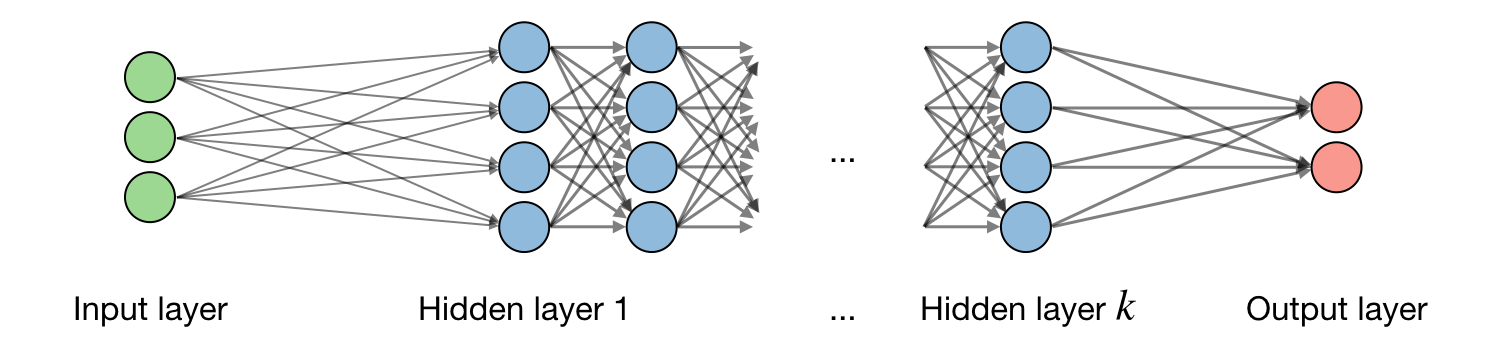
\includegraphics[width=\textwidth]{./fig/neural-networks-architectures.png}
    \caption{neural-networks-architectures}
    \label{fig:neural-networks-architectures}
\end{figure}

We will focus on one node, by noting:

\begin{itemize}
    \item $i$ : the  $i$-th layer of the network
    \item $j$ : the $j$-th hidden units of the layer
    \item $(\vec{x},y)$ : datasets, where $\vec{x}$ is the input and $y$ is the desired output. $\vec{x}\in \mathcal{R}^{n_x}$ has $n_x$ variables
    \item $\vec{w}\in \mathcal{R}^{n_x}$ : weight, each $w$ corresponds to one $x$
    \item $b\in \mathcal{R}$ :  bias
    \item $z$ : output
\end{itemize}

We have:

\begin{tcolorbox}
    \textbf{Forward propagation} (before using the activation function):
   \[
       z_j^{[i]} = (\vec{w}_j^{[i]})^{T} \cdot \vec{x} + b_j^{[i]}
   \]
\end{tcolorbox}

And then, \textbf{activation functions} $\hat{y}=g(z)$ are used at the end of a hidden unit to introduce non-linear complexities to the model.

\begin{figure}[H] %h:当前位置, t:顶部, b:底部, p:浮动页
    \centering
    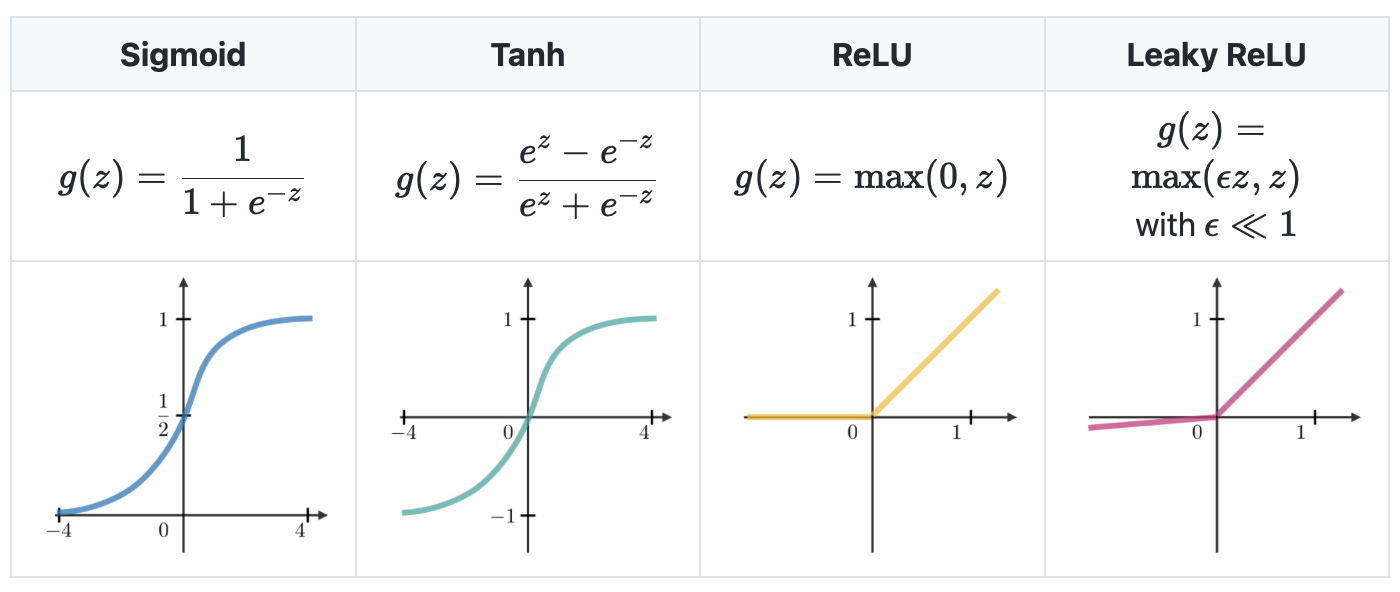
\includegraphics[width=\textwidth]{./fig/activation-functions.png}
    \caption{activation-functions}
    \label{fig:activation-functions}
\end{figure}

Suming up:

\begin{tcolorbox}
    We have dataset $(\vec{x},y)$. With input $x\in \mathcal{R}^{n_x}$, and the help of $\vec{w},b$ and $g$,
\[
    \vec{x} \mapsto z \mapsto \hat{y} = g(z)
\]
    In this way having $\hat{y}$ in our model and $y$ in reality.
\end{tcolorbox}
\subsection{Loss functions}
Here, we are going to measure the difference between $y$ and $\hat{y}$. \textbf{Loss functions} are to measure how well our algorithm is doing based on one single sample.
\begin{tcolorbox}
    \textbf{Cross-entropy loss}:
    \[
    L(\hat{y},y) = -[y\log \hat{y}+(1-y)\log (1-\hat{y})]
    \]
\end{tcolorbox}
\begin{tcolorbox}
    \textbf{Mean squared error loss}:
    \[
    L(\hat{y},y) = (y - \hat{y})^{2}
    \]
\end{tcolorbox}
Also, we have the \textbf{cost function} based on a number of samples:

\begin{tcolorbox}
    \textbf{Cost function}: to measure how well you're doing in the entire training set.

    Here, $n$ means the $n$-th sample, and $m$ is the total number of the samples.
    \[
        J(w,b) = \frac{1}{m} \sum_{n=1}^{m} L(\hat{y}^{[n]}, y ^{[n]})
    \]
\end{tcolorbox}

\subsection{Gradient Descent}

\textbf{Gradient Descent} is based on a convex function and tweaks its parameters iteratively to minimize a given function (here, the cost function) to its local minimum.
\begin{figure}[H]
\begin{minipage}[t]{0.5\linewidth} 
\centering 
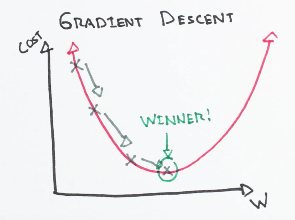
\includegraphics[width=2.0in]{./fig/gradient-descent-1D.png} 
\caption{gradient-descent-1D} 
\label{fig:gradient-descent-1D} 
\end{minipage}% 
\begin{minipage}[t]{0.5\linewidth} 
\centering 
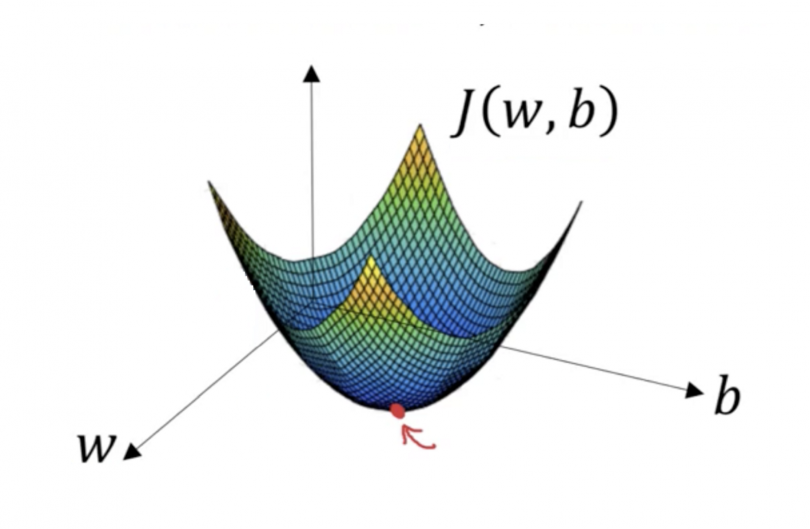
\includegraphics[width=2.5in]{./fig/gradient-descent-3D.png} 
\caption{gradient-descent-3D} 
\label{fig:gradient-descent-3D} 
\end{minipage} 
\end{figure}

We note :
\begin{itemize}
    \item $a$ : current position
    \item $b$ : the next position
    \item $\alpha$ : a waiting factor
    \item $\nabla  f(a)$ : the direction of the steepest descent at $a$
\end{itemize}
\begin{tcolorbox}
    What \textbf{gradient descent} does:
    \[
        b = a - \alpha \cdot \nabla f(a)
    \]
\end{tcolorbox}

We define $\alpha$ as the \textbf{learning rate}, which indicates at which space the weights get updated.

It is very important for us to select a appropriate value of $\alpha$.
\begin{figure}[H] %h:当前位置, t:顶部, b:底部, p:浮动页
    \centering
    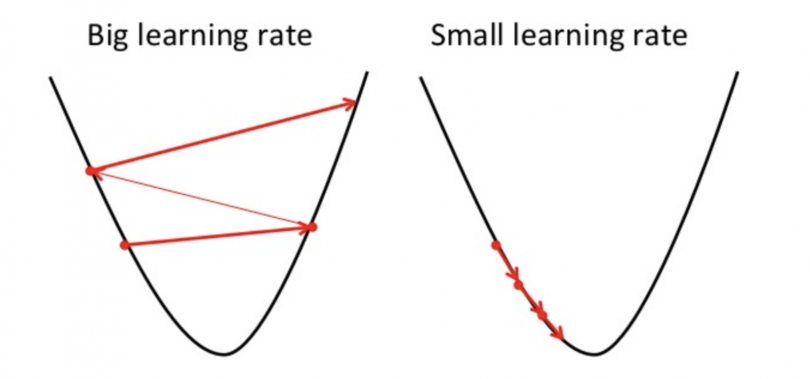
\includegraphics[width=0.5\textwidth]{./fig/gradient-descent-learning-rate.png}
    \caption{gradient-descent-learning-rate}
    \label{fig:gradient-descent-learning-rate}
\end{figure}

After several iterations by repeating the method until $|\nabla f|< \varepsilon$, which means it has converged, then stop.

\subsection{Backpropogation}

\textbf{Backpropogation} is an algorithm for supervised learning of artificial neural networks using \textbf{gradient descent}.

Here, we have :
\[
\hat{y} = g(z), z = w^{T}x+b
\]

For one single node with $(x\in \mathcal{R}^{n_x},y)$, we focus on one variable $w_k$ which correspond to $x_k \in \{x_1, \ldots,x_{n_x}\}$ by using the \textbf{chain rule of differentiation}:
\begin{align*}
    \nabla_w = \frac{\partial L(\hat{y},y)}{\partial w_k}
    &= \frac{\partial L(\hat{y},y)}{\partial \hat{y}} \cdot \frac{\text{d}\hat{y}}{\text{d}z} \cdot \frac{\partial z}{\partial w_k} \\
    &= \frac{\partial L(\hat{y},y)}{\partial z} \cdot x_k 
\end{align*}

If $g$ is the sigmoid function, and the loss function is the cross-entropy loss function, then for each $w_k$,
\[
\nabla_w =\frac{\partial L(\hat{y},y)}{\partial w_k} = (\hat{y}-y) \cdot x_k
\]
\[ \begin{cases}
    w_k &:= w_k - \alpha(\hat{y}-y)x_k \\
    b_k &:= b_k - \alpha(\hat{y}-y)
\end{cases}
\]

\begin{tcolorbox}
$w$ and $b$ are updated as follows :
\begin{enumerate}
    \item Take a batch of training data
    \item Perform \textbf{forward propagation} to obtain the corresponding loss
    \item \textbf{Backpropagate} the loss to get the gradients
    \item Use the gradients to update the weights of the network
\end{enumerate}
\end{tcolorbox}
The whole process is:
\begin{verbatim}
    ---Initializing---
    g = (an activation function)
    J = 0
    L = (Cross-entropy loss)
    For p = 1 to (the total number of inputs)
        dw_p = 0
        w_p = (random but appropriate number)
    db = 0
    alpha = (learning rate)

    ---For all the samples---
    For n = 1 to m
        ---Forward Propagation---
        z = wx + b
        a = g(z)
        J += L(a,y)
        ---Backpropagation---
        dz = (after calculation)
        For p = 1 to (the total number of inputs)
            dw_p += x_p * dz
        db += dz
    
    ---Update w and b by using the gradients---
    J /= m
    For p = 1 to (the total number of inputs)
        dw_p /= m
        w_p := w_p - alpha * dw_p
    b := b - alpha * db
\end{verbatim}

\end{document}